\section{Class diagrams}
\twopagepicture{b}{l}{figures/CommonLayer}{Class diagram common layer}
\subsection{Common layer}
The \texttt{CommonLayer} is shown in figure 2. The design of the classes are in mind that it can be shared in between layers and it can be serialized (written to file). Hence the class diagram follow the constraints that it can't use any interfaces or that there is a circular reference (it has to look like a tree). Notice that the 
\texttt{PedestrianEntity} and the \texttt{CarEntity} are in an \texttt{ObservableCollection} and have observable attributes. When the simulation is running the view will be be notified when attributes are changed.

\subsubsection{Entities}
The classes of the common layer all end with *Entity. An entity in this program is a serializable object which will be used between all layers. The objects contain no operations, creating such objects can be best done using the object initializer (instead of the constructor). For example take the class point with values X and Y, can be created by \texttt{new Point \{ X = 100, Y = 200 \};}  

\subsection{View layer}
In figure \ref{fig:pres} the class diagram of the view layer is shown. Inside of the view we do not use the usual \texttt{Graphics} used in Forms application to draw on the screen but instead a \texttt{Canvas} to draw on the screen. A lot of the drawing is already handled and we have especially bind the right values.

\subsubsection{UserControl}
An UserControl is a Control shown on the screen hence it also has a View. The UserControl has logic for displaying certain elements on the screen. The UserControl observes the Entities. For example when the value of \texttt{CarEntity} has changed then the \texttt{CarUserControl} related to that also has to move itself.

\subsection{ViewModel}
A \texttt{ViewModel} is an object which the program can bind to the View of the Window, and then these values are shown on the screen. The values can also be altered for example when put in a TextBox. The responsibility of serializing the values is with WPF, hence we don't need to check if the values we receive are indeed for example an integer. Hence \texttt{ViewModel} can also be observed using the \texttt{PropertyChanged} event, then the according entities can also be updated. 

\subsection{Business Layer}
In figure \ref{fig:bus} the class diagram of the business layer is shown. We choose to make operations for adding and deleting components instead of using an observable collection since by using operations is more simple to maintain business rules. 

\subsection{Data Layer}
In figure \ref{fig:data} the class diagram of the data layer is shown. The data layer does not show concrete implementation since the classes don't require to have a state.

\newpage
\begin{figure}[!ht]
	\centering
	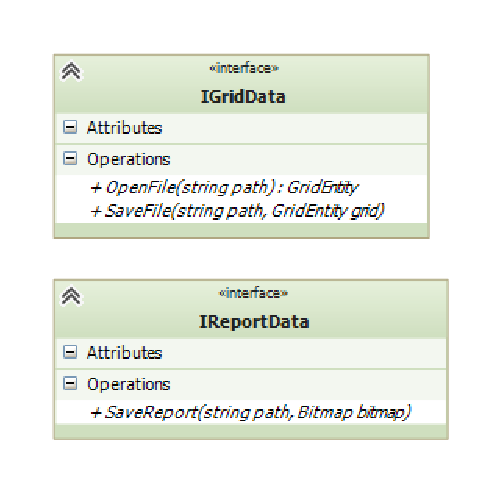
\includegraphics{figures/DataLayer}
	\caption{Class diagram data access layer}
	\label{fig:data}
\end{figure}



\begin{landscape}
	\begin{figure}[!ht]
		\centering
		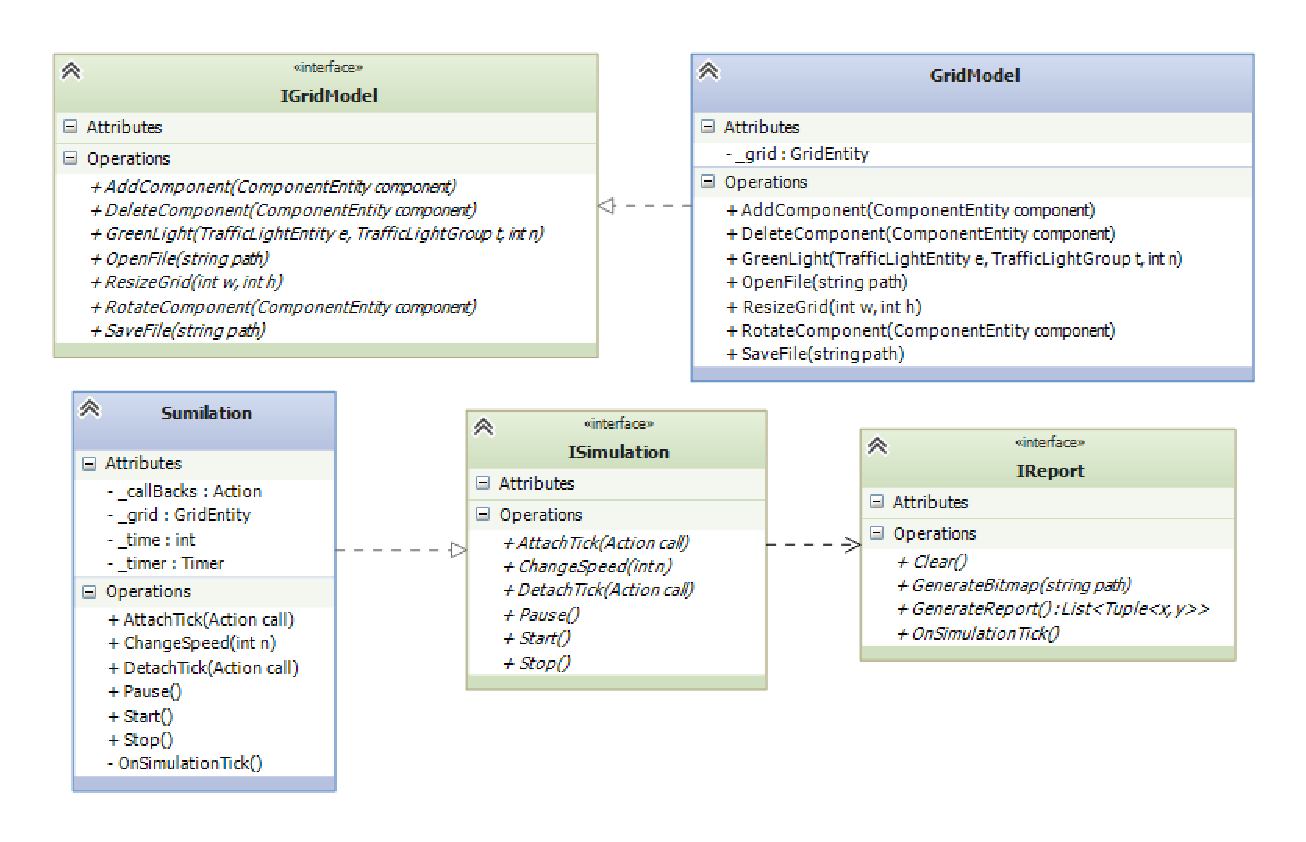
\includegraphics[height=\textheight]{figures/BusinessLayer}
		\caption{Class diagram business layer}
		\label{fig:bus}
	\end{figure}
\end{landscape}

\begin{landscape}
	\begin{figure}[!ht]
		\centering
		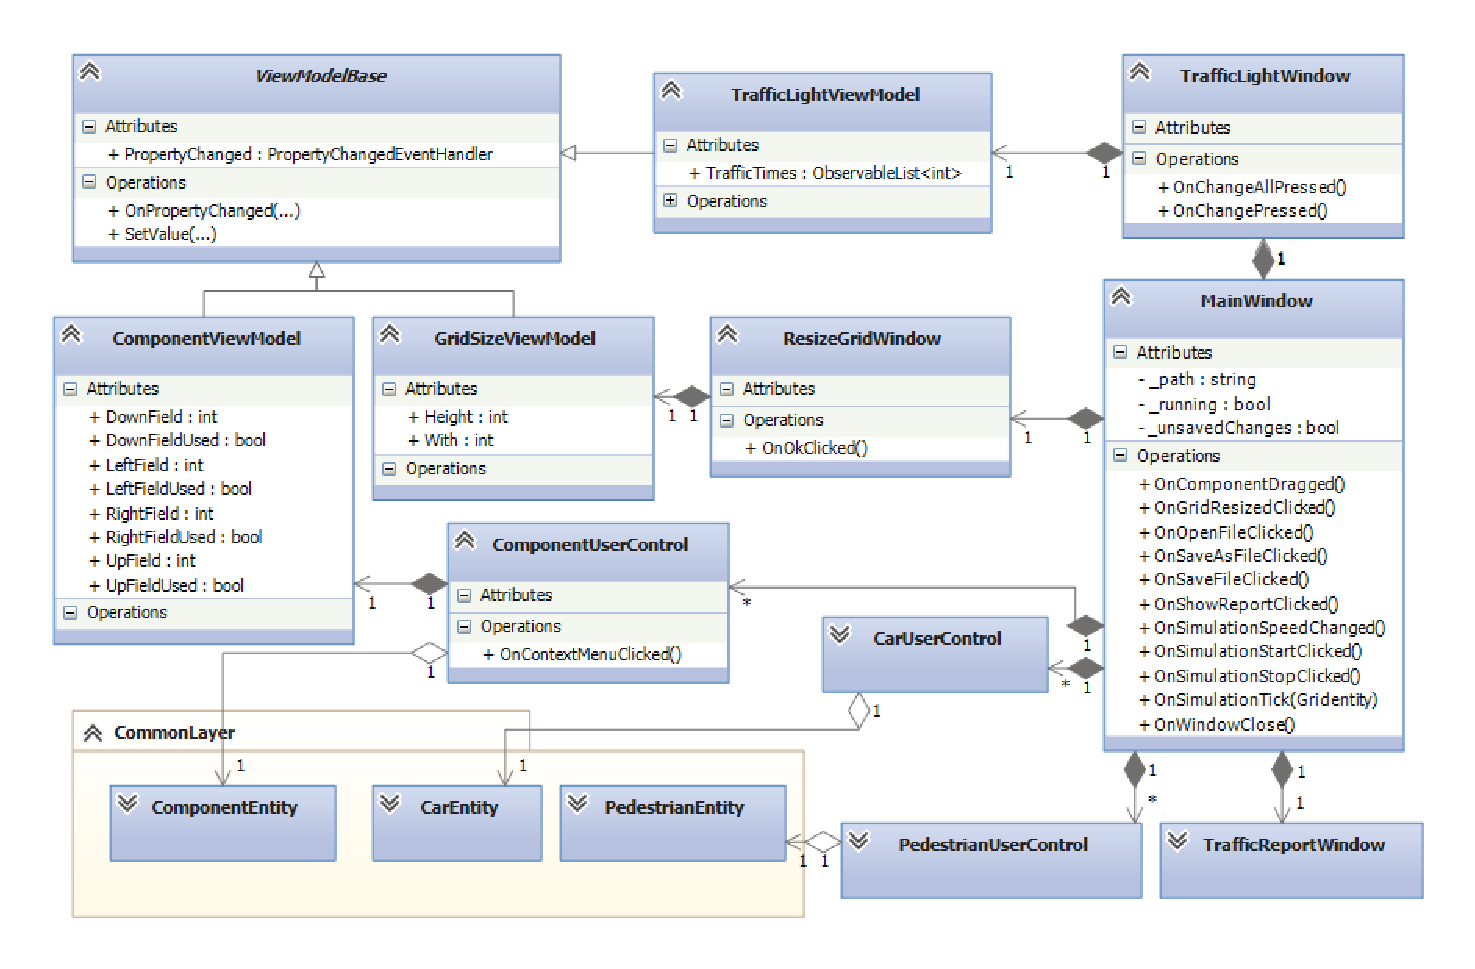
\includegraphics[height=\textheight]{figures/PresentationLayer}
		\caption{Class diagram view layer}
		\label{fig:pres}
	\end{figure}
\end{landscape}




